\documentclass[a4paper]{article}

\usepackage[utf8]{inputenc}
\usepackage[T1]{fontenc}
\usepackage{textcomp}
\usepackage[italian]{babel}
\usepackage{amsmath, amssymb}
\usepackage{booktabs,xltabular}
\usepackage{amsfonts}
\usepackage{cancel}
\usepackage{mdframed}
\usepackage{makecell}
\usepackage{float}
\usepackage{xcolor}
\usepackage{listings}
\usepackage{graphicx}
\usepackage{tikz}
\usetikzlibrary{shapes, arrows, automata, petri, decorations.pathreplacing, positioning, calc}
\usepackage{circuitikz}
\usepackage[label=corner]{karnaugh-map}
\graphicspath{{./figures/}}

\usepackage{ntheorem}
\newtheorem{theorem}{Teorema}

\usepackage{import}
\usepackage{pdfpages}
\usepackage{transparent}
\usepackage{xcolor}

\usepackage{hyperref}
\hypersetup{
    colorlinks=false,
}

% Code blocks
\definecolor{codegreen}{rgb}{0,0.6,0}
\definecolor{codegray}{rgb}{0.5,0.5,0.5}
\definecolor{codepurple}{rgb}{0.58,0,0.82}
\definecolor{backcolour}{rgb}{0.95,0.95,0.95}

\lstdefinestyle{mystyle}{
	backgroundcolor=\color{backcolour},
	commentstyle=\color{codegreen},
	keywordstyle=\color{magenta},
	numberstyle=\tiny\color{codegray},
	stringstyle=\color{codepurple},
	basicstyle=\ttfamily\footnotesize,
	breakatwhitespace=false,
	breaklines=true,
	captionpos=b,
	keepspaces=true,
	numbers=left,
	numbersep=5pt,
	showspaces=false,
	showstringspaces=false,
	showtabs=false,
	tabsize=2
}

\lstset{style=mystyle}

\usepackage{color}

\definecolor{dkgreen}{rgb}{0,0.6,0}
\definecolor{gray}{rgb}{0.5,0.5,0.5}
\definecolor{mauve}{rgb}{0.58,0,0.82}

\lstset{frame=tb,
	aboveskip=3mm,
	belowskip=3mm,
	showstringspaces=false,
	columns=flexible,
	basicstyle={\small\ttfamily},
	numbers=none,
	numberstyle=\tiny\color{gray},
	keywordstyle=\color{blue},
	commentstyle=\color{dkgreen},
	stringstyle=\color{mauve},
	breaklines=true,
	breakatwhitespace=true,
	tabsize=3
}

\usepackage{import}
\usepackage{pdfpages}
\usepackage{transparent}
\usepackage{xcolor}



% Useful definitions frame
\theoremstyle{break}
\theoremheaderfont{\bfseries}
\newmdtheoremenv[%
	linecolor=gray,leftmargin=0,%
	rightmargin=0,
	innertopmargin=8pt,%
	innerbottommargin=8pt,
	ntheorem]{define}{Definizioni utili}[section]

% Example frame
\theoremstyle{break}
\theoremheaderfont{\bfseries}
\newmdtheoremenv[%
	linecolor=gray,leftmargin=0,%
	rightmargin=0,
	innertopmargin=8pt,%
	innerbottommargin=8pt,
	ntheorem]{example}{Esempio}[section]

% Important definition frame
\theoremstyle{break}
\theoremheaderfont{\bfseries}
\newmdtheoremenv[%
	linecolor=gray,leftmargin=0,%
	rightmargin=0,
	backgroundcolor=gray!40,%
	innertopmargin=8pt,%
	innerbottommargin=8pt,
	ntheorem]{definition}{Definizione}[section]

% Exercise frame
\theoremstyle{break}
\theoremheaderfont{\bfseries}
\newmdtheoremenv[%
	linecolor=gray,leftmargin=0,%
	rightmargin=0,
	innertopmargin=8pt,%
	innerbottommargin=8pt,
	ntheorem]{exercise}{Esercizio}[section]

% figure support
\usepackage{import}
\usepackage{xifthen}
\pdfminorversion=7
\usepackage{pdfpages}
\usepackage{transparent}
\newcommand{\incfig}[1]{%
	\def\svgwidth{\columnwidth}
	\import{./figures/}{#1.pdf_tex}
}

% FSM tikz
\tikzset{
    place/.style={
        circle,
        thick,
        draw=black,
        minimum size=6mm,
    },
        state/.style={
        circle,
        thick,
        draw=blue!75,
        fill=blue!20,
        minimum size=6mm,
    },
}

\pdfsuppresswarningpagegroup=1

\begin{document}

\begin{titlepage}
	\begin{center}
		\vspace*{1cm}

		\Huge
		\textbf{Probabilità e Statistica\\Esercizi}

		\vspace{0.5cm}
		\LARGE
		UniVR - Dipartimento di Informatica

		\vspace{1.5cm}

		\textbf{Fabio Irimie}

		\vfill


		\vspace{0.8cm}


		2° Semestre 2023/2024

	\end{center}
\end{titlepage}


\tableofcontents
\pagebreak

\section{Introduzione}
Il problema principale che bisogna affrontare è la comunicazione tra 2 calcolatori,
cioè lo scambio di informazioni. Per far comunicare 2 calcolatori c'è bisogno di
alcuni requisiti:
\begin{enumerate}
  \item \textbf{Protocollo}: È un insieme di regole che sovraintende alla comunicazione,
    in cui si definiscono:
    \begin{itemize}
      \item Il formato dei messaggi
      \item Le azioni da intraprendere nel gestire i messaggi stessi
    \end{itemize}
    Questo perchè per comunicare tutti devono "parlare la stessa lingua".

  \item \textbf{Architettura di rete}: Come, fisicamente, trasportare i messaggi
\end{enumerate}

\begin{figure}[H]
  \begin{example}
    Prendiamo ad esempio la scrittura e la spedizione delle lettere. Ci sono 2
    utenti che vogliono scambiare delle lettere.
    
    Per gestire il trasporto della
    lettera essa viene messa all'interno di una \textbf{busta}, che contiene informazioni
    su dove deve essere spedita. Una volta inbustata, va imbucata in una cassetta 
    delle lettere da cui poi verrà prelevata e mandata alla cassetta delle lettere 
    del secondo utente dalla \textbf{rete} di distribuzione degli uffici postali.

    L'utente poi preleverà la lettera dalla cassetta delle lettere e dopo aver
    controllato le informazioni sulla busta, la aprirà e leggerà il contenuto.
    \begin{figure}[H]
      \begin{center}
        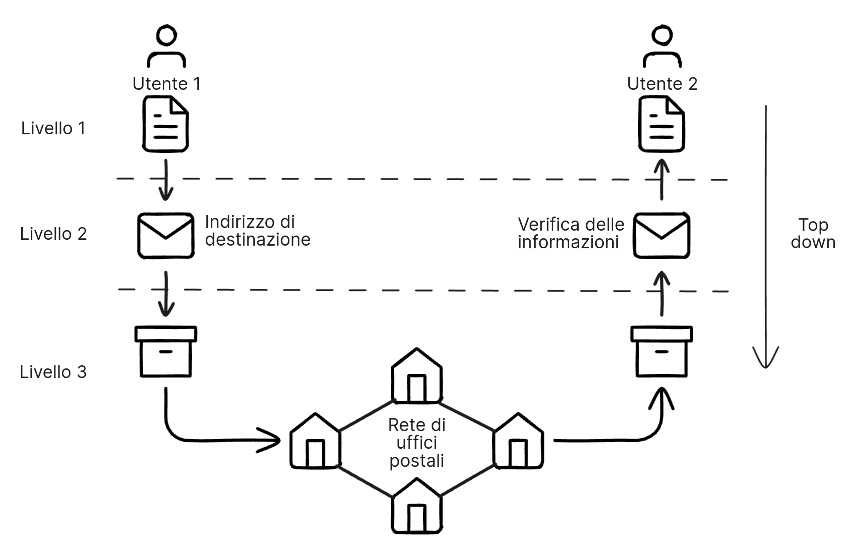
\includegraphics[width=0.95\textwidth]{rete-postale}
      \end{center}
      \caption{Esempio di comunicazione tra 2 utenti}
    \end{figure}

    Il \textbf{Protocollo} è il linguaggio utilizzato per comunicare tra i 2
    utenti, mentre l'\textbf{Architettura di rete} è tutta quella infrastruttura
    che trasporta il messaggio tra i 2 utenti.
  \end{example}
\end{figure}

\noindent
La rappresentazione dei sistemi di comunicazione di solito viene fatta nella modalità
\textbf{top-down}, cioè si parte dal livello applicativo, quello più alto, fino a scendere
nei livelli più bassi in cui si trova la vera e propria architettura della rete.
\end{document}
